\documentclass[
	10pt,								% globale Schriftgröße
	parskip=half-,						% setzt Absatzabstand hoch
	paper=a4,							% Format
	english,
	appendixprefix=true					% lädt Sprachpakete
	]{scrartcl}							% Dokumentenklasse
%\linespread{1.2} % Increase line spacing
% //////////////////// Pakete laden ////////////////////
\usepackage{amsmath}			% MUSS vor fontspec geladen werden
\usepackage{mathtools}			% modifiziert amsmath
\usepackage{amssymb}			% mathematische symbole, für \ceckmarks
\usepackage{amsthm}				% für proof
\usepackage{mathrsfs}			% für \mathscr
\usepackage{latexsym}
\usepackage{marvosym}				% für Lightning

%%% to allow custom headings
\usepackage{titlesec}
% to change titles font family
\usepackage{titling}

\usepackage{fontspec} 			% funktioniert nur mit den neueren Compilern z.B. XeLaTeX
\usepackage{microtype}			% für bessere Worttrennung
\usepackage[ngerman]{babel} 	% Spracheinstellung
\usepackage{lmodern}			% verändert verwendete Schriftart, damit sie weniger pixelig ist

\usepackage{verbatim}
\usepackage{listings}			% Für Quellcode

\usepackage{graphicx}
\usepackage{subcaption}
\usepackage{tabularx}			% für Tabellen mit gleicher Spaltenbreite und automatischen Umbrüchen
\usepackage{fullpage}
\usepackage{multirow}			% für multirow in tabulars
\usepackage{rotate}
\usepackage[cmyk,table]{xcolor} % um Farben zu benutzen, kann mehr als das Paket color
\usepackage[					% Verlinkungen
	colorlinks,					% farbige Schrift, statt farbiger Rahmen
	linktocpage,				% verlinkt im Abb.Verzeichnis Seitenzahl statt Bildunterschrift
	linkcolor=blue,				% setzt Farbe der Links auf blau
	urlcolor=blue	
	]{hyperref}					% nur für digitale Anwendungen, url = "http://www.example.com"
\usepackage{url}				% für Webadressen wie e-mail usw.: "\url{http://www.example.com}"
\urlstyle{sf}

\usepackage{enumerate}			% für versch. Aufzählungezeichen wie z.B. a)
\usepackage{xspace}				% folgt ein Leerzeichen nach einem \Befehl, wird es nicht verschluckt.
\usepackage{cancel}				% für das Durchstreichen u.a. in Matheformeln mit \cancel
\usepackage{float}              % zum Forcieren der Position von figure-Umgebungen

% Change font of document
\setsansfont{Source Sans Pro}
\setmainfont{Source Sans Pro}
% font declaration and title settings
\newfontfamily\headingfont[]{Source Sans Pro Light}
\titleformat{\chapter}[display]
  {\huge\headingfont}{\chaptertitlename\ \thechapter}{26pt}{\Huge}
\titleformat*{\section}{\LARGE\headingfont}
\titleformat*{\subsection}{\Large\headingfont}
\renewcommand{\maketitlehooka}{\headingfont}

\newfontfamily\ttfamily[]{Roboto Mono}
% zum Zeichnen (u.a. von Graphen)
\usepackage{fp}
\usepackage{tikz}
\usetikzlibrary{tikzmark}			% für \tikzmark{toRemember}
\usetikzlibrary{positioning}	% verbesserte Positionierung der Knoten
\usetikzlibrary{automata}		% für Automaten (GTI)
\usetikzlibrary{arrows}
\usetikzlibrary{shapes}
\usetikzlibrary{decorations.pathmorphing}
\usetikzlibrary{decorations.pathreplacing}
\usetikzlibrary{decorations.shapes}
\usetikzlibrary{decorations.text}

% //////////////////// Syntaxhighlighting ////////////////////
\lstloadlanguages{Python, Haskell, [LaTeX]TeX, Java}
\lstset{
   basicstyle=\footnotesize\ttfamily,	% \scriptsize the size of the fonts that are used for the code
   backgroundcolor = \color{bgcolour},	% legt Farbe der Box fest
   breakatwhitespace=false,	% sets if automatic breaks should only happen at whitespace
   breaklines=true,			% sets automatic line breaking
   captionpos=t,				% sets the caption-position to bottom, t for top
   commentstyle=\color{codeblue}\ttfamily,% comment style
   frame=single,				% adds a frame around the code
   keepspaces=true,			% keeps spaces in text, useful for keeping indentation
							% of code (possibly needs columns=flexible)
   keywordstyle=\bfseries\ttfamily\color{codepurple},% keyword style
   numbers=left,				% where to put the line-numbers;
   							% possible values are (none, left, right)
   numberstyle=\tiny\color{codegreen},	% the style that is used for the line-numbers
   numbersep=5pt,			% how far the line-numbers are from the code
   stepnumber=1,				% nummeriert nur jede i-te Zeile
   showspaces=false,			% show spaces everywhere adding particular underscores;
							% it overrides 'showstringspaces'
   showstringspaces=false,	% underline spaces within strings only
   showtabs=false,			% show tabs within strings adding particular underscores
   flexiblecolumns=false,
   tabsize=1,				% the step between two line-numbers. If 1: each line will be numbered
   stringstyle=\color{orange}\ttfamily,	% string literal style
   numberblanklines=false,				% leere Zeilen werden nicht mitnummeriert
   xleftmargin=1.2em,					% Abstand zum linken Layoutrand
   xrightmargin=0.4em,					% Abstand zum rechten Layoutrand
   aboveskip=2ex, 
}

\lstdefinestyle{py}{
   language=Python,
}
\lstdefinestyle{hs}{
   language=Haskell,
}
\lstdefinestyle{tex}{
	language=[LaTeX]TeX,
	escapeinside={\%*}{*)},     % if you want to add LaTeX within your code
	texcsstyle=*\bfseries\color{blue},% hervorhebung der tex-Schlüsselwörter
	morekeywords={*,$,\{,\},\[,\],lstinputlisting,includegraphics,
	rowcolor,columncolor,listoffigures,lstlistoflistings,
	subsection,subsubsection,textcolor,tableofcontents,colorbox,
	fcolorbox,definecolor,cellcolor,url,linktocpage,subtitle,
	subject,maketitle,usetikzlibrary,node,path,addbibresource,
	printbibliography},% if you want to add more keywords to the set
     numbers=none,
     numbersep=0pt,
     xleftmargin=0.4em,
}

\lstdefinestyle{java}{
	language=Java,
	extendedchars=true,		% lets you use non-ASCII characters;
   						% for 8-bits encodings only, does not work with UTF-8
}

\lstdefinelanguage[x64]{Assembler}     % add a "x64" dialect of Assembler
   [x86masm]{Assembler} % based on the "x86masm" dialect
   % with these extra keywords:
   {morekeywords={CDQE,CQO,CMPSQ,CMPXCHG16B,JRCXZ,LODSQ,MOVSXD, %
                  POPFQ,PUSHFQ,SCASQ,STOSQ,IRETQ,RDTSCP,SWAPGS, %
                  rax,rdx,rcx,rbx,rsi,rdi,rsp,rbp, %
                  r8,r8d,r8w,r8b,r9,r9d,r9w,r9b}
}					% for 8-bits encodings only, does not work with UTF-8

\lstdefinestyle{c}{
	language=c,
	extendedchars=true,		% for 8-bits encodings only, does not work with UTF-8
}

% //////////////////// eigene Kommandos ////////////////////
\newcommand\FU{Freie Universität Berlin\xspace}% benötigt package xspace
\newcommand\gdw{g.\,d.\,w.\xspace}
\newcommand\oBdA{o.\,B.\,d.\,A.\xspace}
\newcommand{\Eu}{\texteuro}
\newcommand\N{\mathbb{N}\xspace}
\newcommand\Q{\mathbb{Q}\xspace}
\newcommand\R{\mathbb{R}\xspace}
\newcommand\Z{\mathbb{Z}\xspace}
\newcommand\ohneNull{\ensuremath{\backslash\lbrace 0\rbrace}}% \{0}
\let\dhALT\dh	% Schreibt Befehl \dh in \dhALT um
\renewcommand\dh{d.\,h.\xspace}	%renew überschreibt command \dh
\newcommand\Bolt{\;\text{\LARGE\raisebox{-0.3em}{\Lightning}\normalsize}\xspace}% Blitz
\newcommand\zz{\ensuremath{\raisebox{+0.25ex}{Z}% zu zeigen
			\kern-0.4em\raisebox{-0.25ex}{Z}%
			\;\xspace}}
\newcommand{\from}{\ensuremath{\colon}}
\newcommand{\floor}[1]{\lfloor{#1}\rfloor}
\newcommand{\ceil}[1]{\lceil{#1}\rceil}
 \renewcommand{\L}{\ensuremath{\mathcal{L}}\xspace}
 \renewcommand{\P}{\ensuremath{\mathcal{P}}\xspace}
 \newcommand{\NL}{\ensuremath{\mathcal{N}\kern-0.2em\mathcal{L}}\xspace}
 \newcommand{\NP}{\ensuremath{\mathcal{NP}}\xspace}

% //////////////////// Mathefunktionen ////////////////////
\DeclareMathOperator{\Landau}{\mathcal{O}}
\DeclareMathOperator{\True}{True}
\DeclareMathOperator{\False}{False}

% //////////////////// eigene Theoreme ////////////////////
\newtheorem{theorem}{Satz}
\newtheorem{corollary}[theorem]{Folgerung}
\newtheorem{lemma}[theorem]{Lemma}
\newtheorem{observation}[theorem]{Beobachtung}
\newtheorem{definition}[theorem]{Definition}
\newtheorem{Literatur}[theorem]{Literatur}
% konfiguriert proof
\makeatletter
\newenvironment{Proof}[1][\proofname]{\par
  \pushQED{\qed}%
  \normalfont \topsep6\p@\@plus6\p@\relax
  \trivlist
  \item[\hskip\labelsep
%         \itshape
        \bfseries
    #1\@addpunct{.}]\ignorespaces
}{%
  \popQED\endtrivlist\@endpefalse
}
\makeatother

% //////////////////// eigene Farben ////////////////////
\let\definecolor=\xdefinecolor
\definecolor{FUgreen}{RGB}{153,204,0}
\definecolor{FUblue}{RGB}{0,51,102}

\definecolor{middlegray}{rgb}{0.5,0.5,0.5}
\definecolor{lightgray}{rgb}{0.8,0.8,0.8}
\definecolor{orange}{rgb}{0.8,0.3,0.3}
\definecolor{azur}{rgb}{0,0.7,1}
\definecolor{yac}{rgb}{0.6,0.6,0.1}
\definecolor{Pink}{rgb}{1,0,0.6}

\definecolor{bgcolour}{rgb}{0.97,0.97,0.97}
\definecolor{codegreen}{rgb}{0,0.6,0}
\definecolor{codegray}{rgb}{0.35,0.35,0.35}
\definecolor{codepurple}{rgb}{0.58,0,0.82}
\definecolor{codeblue}{rgb}{0.4,0.5,1}

% //////////////////// eigene Settings ////////////////////

\textheight = 230mm		% Höhe des Satzspiegels / Layouts
\footskip = 10ex			% Abstand zw. Fußzeile und Grundlinie letzter Textzeile
\parindent 0pt			% verhindert Einrückung der 1. Zeile eines Absatzes
\setkomafont{sectioning}{\rmfamily\bfseries}% setzt Ü-Schriften in Serifen, {disposition}

\usepackage{booktabs}
\usepackage[babel, german=quotes]{csquotes} % einfache Handhabung von quotations
\usepackage[backend=biber]{biblatex} %biblatex mit biber laden
\ExecuteBibliographyOptions{
sorting=nyt, %Sortierung Autor, Titel, Jahr
bibwarn=true, %Probleme mit den Daten, die Backend betreffen anzeigen
isbn=false, %keine isbn anzeigen
url=false %keine url anzeigen
}											% bindet Header ein

\renewcommand{\arraystretch}{1.2} % more whitespace in tables
\usepackage{array} % Being able to format columns of tables
\addbibresource{lit.bib} %Bibliographiedateien laden

\begin{document}
 
\title{Final Course Assignment \\ }%replace X with the appropriate number
\author{Mark Niehues, Stefaan Hessmann \\ %replace with your name
Mathematical Aspects in Machine Learning} %if necessary, replace with your course title

\maketitle
 
\section{Introduction}
In the past course we dealt with the broad mathematical foundations of machine learning. To get an idea of what the consequences of those mathematical theorems and approaches are and to get in touch with the standard Python tools, we have evaluated an comparatively easy data science example found on \url{kaggle.com}. The example dataset \cite{Kaggle2017} consists of the historic passenger records of the disastrous Titanic maiden voyage in 1912. The goal in this challenge was to predict if a passenger survived the accident based on informations like for example age, sex and payed ticket fare. Therefore it is in terms of machine learning a \textit{classification problem} with two classes: survived and not survived.

Inspired by sample solutions from the website, we first took a deeper look on the dataset and tried to select the most significant influences by reviewing the statistical properties of the dataset. In the following we implemented an naive Sequential Minimal Optimization (SMO) algorithm and ran a few tests with them in order to finally compare the results with other machine learning algorithms.

\section{Applying Machine Learning Methods on the Titanic Disaster}
\subsection{Dataset}
The given dataset consists of a CSV-file containing data of 891 passengers. The dataset contains an ID for every passenger, a label if the passenger has survived the disaster and the features that are described in table \ref{tab:features}. It can be noticed that some of the features are incomplete.

\begin{table}
\caption{Features and their amount of missing data.}
\begin{tabular}{>{\bfseries}l l l}
PassengerId & Unique ID for every passenger & 0.0 \%\\
Survived & Survived (1) or died (0) & 0.0 \% \\
Pclass & Passenger's class & 0.0 \% \\
Name & Passenger's name & 0.0 \% \\
Sex & Passenger's sex & 0.0 \% \\
Age & Passenger's age & \textbf{19.87 \%} \\
SibSp & Number of siblings/spouses aboard & 0.0 \% \\
Parch & Number of parents/children aboard & 0.0 \% \\
Ticket & Ticket number & 0.0 \% \\
Fare & Ticket-price & 0.0 \% \\
Cabin & Number of the passenger's cabin & \textbf{77.10 \%} \\
Embarked & Port of embarkation & \textbf{0.22 \%} \\
\end{tabular}
\centering
\label{tab:features}
\end{table}

After loading the dataset, it is necessary to process the data for our learning machine. Therefore the different features will be investigated to select meaningful features and the missing data needs to be handled. There were some features that could be used for supervised training in a more or less straight forward way. First, the sex-feature which separates the passengers in male and female. We can conclude from fig .\ref{fig:sexfeat} that 'Sex' seems to be a meaningful feature for the learning machine as females had a much higher probability to survive.\\
Secondly, the wealth of a passenger expressed in the passengers Class and the fare he paid for the ticket has positive influence on his chance to survive. The fare feature was categorized into three groups of similar survival rates to permit overfitting (fig. \ref{fig:farefeat}). Surprisingly the port of embarkation also correlates with the survival rate as can be seen in figure \ref{fig:embarkationfeat}. Passengers that joined the Titanic at Cherbourg had higher survival chances that people who embarked at other harbours. The other features were engineered in a slightly more advanced way as described below.

\begin{figure}
    \centering
    \begin{subfigure}[b]{0.3\textwidth}
     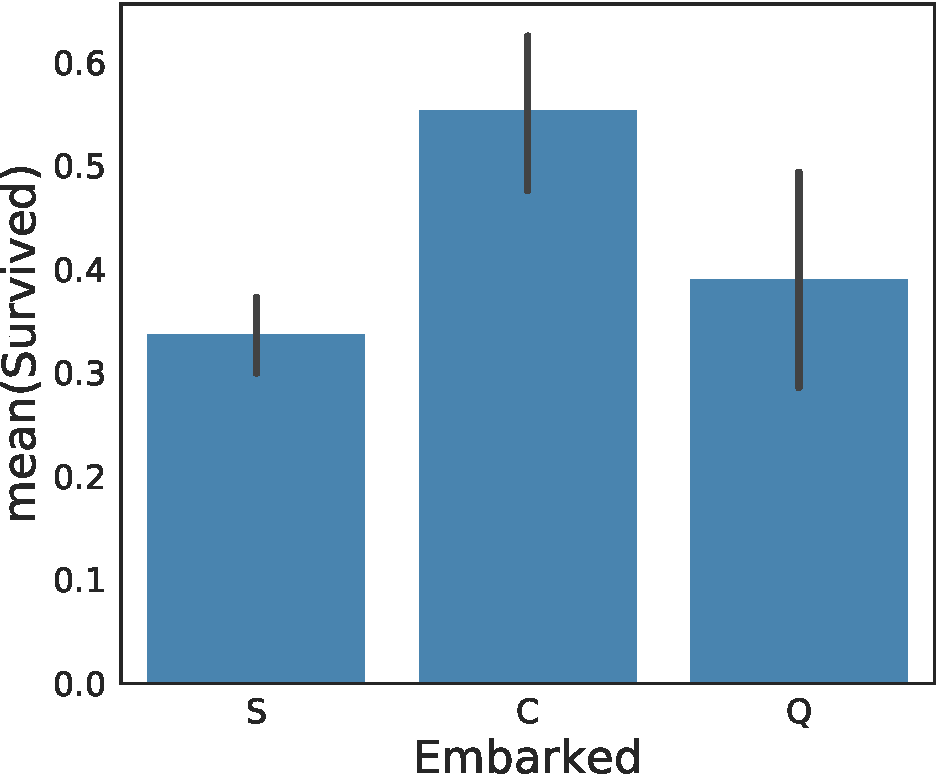
\includegraphics[width=\textwidth]{media_saved/embarkation_survived}
     \caption{Survival probability correlated with ports of embarkation. \\}
     \label{fig:embarkationfeat}
    \end{subfigure}
    \quad
    \begin{subfigure}[b]{0.3\textwidth}
        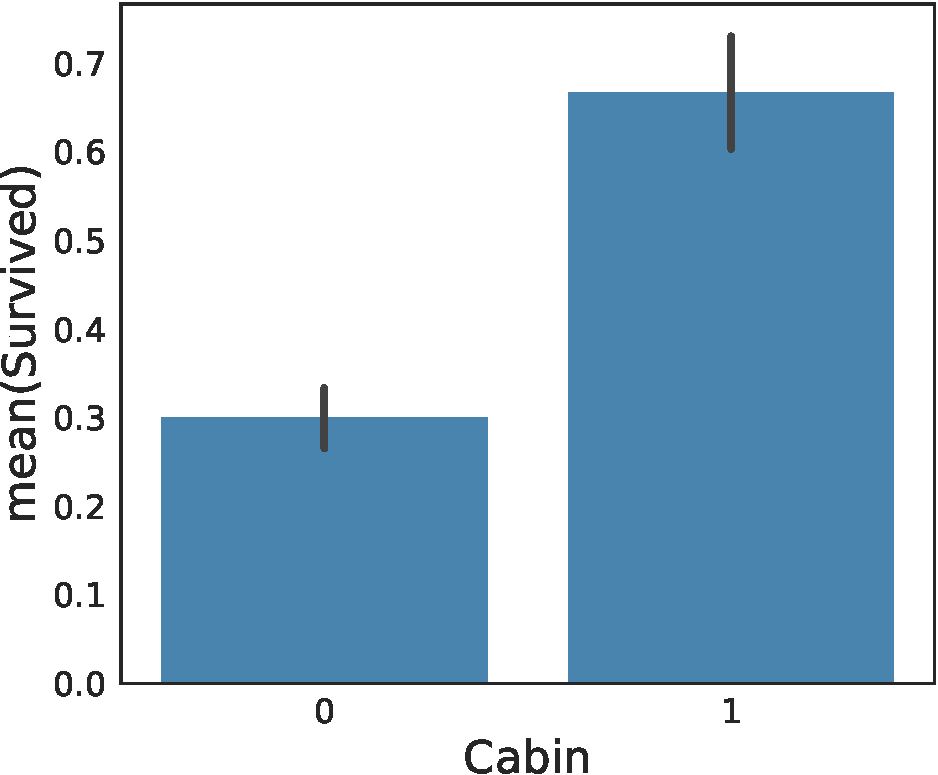
\includegraphics[width=\textwidth]{media_saved/cabin_survived}
     \caption{Correlation between preservation of cabin number and survival rate.}
     \label{fig:cabinfeat}
    \end{subfigure}
    \quad
    \begin{subfigure}[b]{0.3\textwidth}
        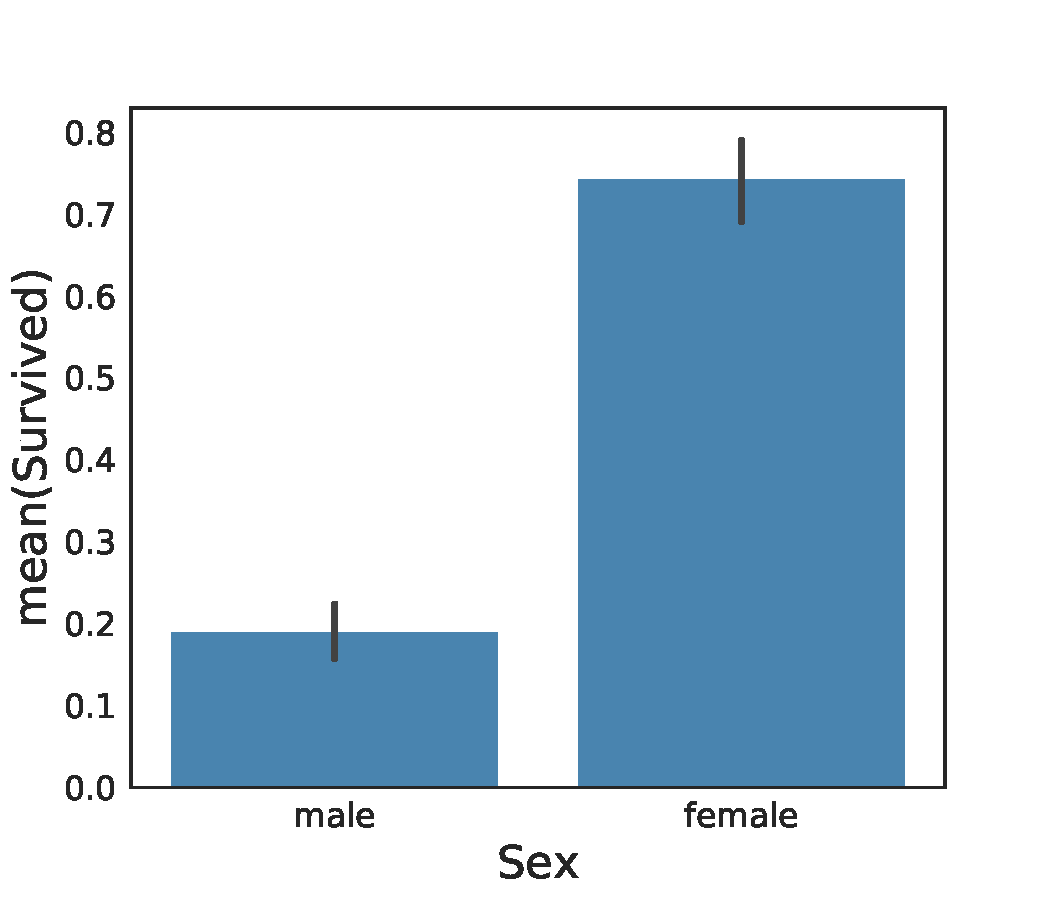
\includegraphics[width=\textwidth]{media_saved/sex_survived}
  \caption{Survival probability depending on the passenger's sex.\\}
  \label{fig:sexfeat}
    \end{subfigure}
    \caption{Relation between several features and the survival rate.}
\end{figure}


\begin{figure}
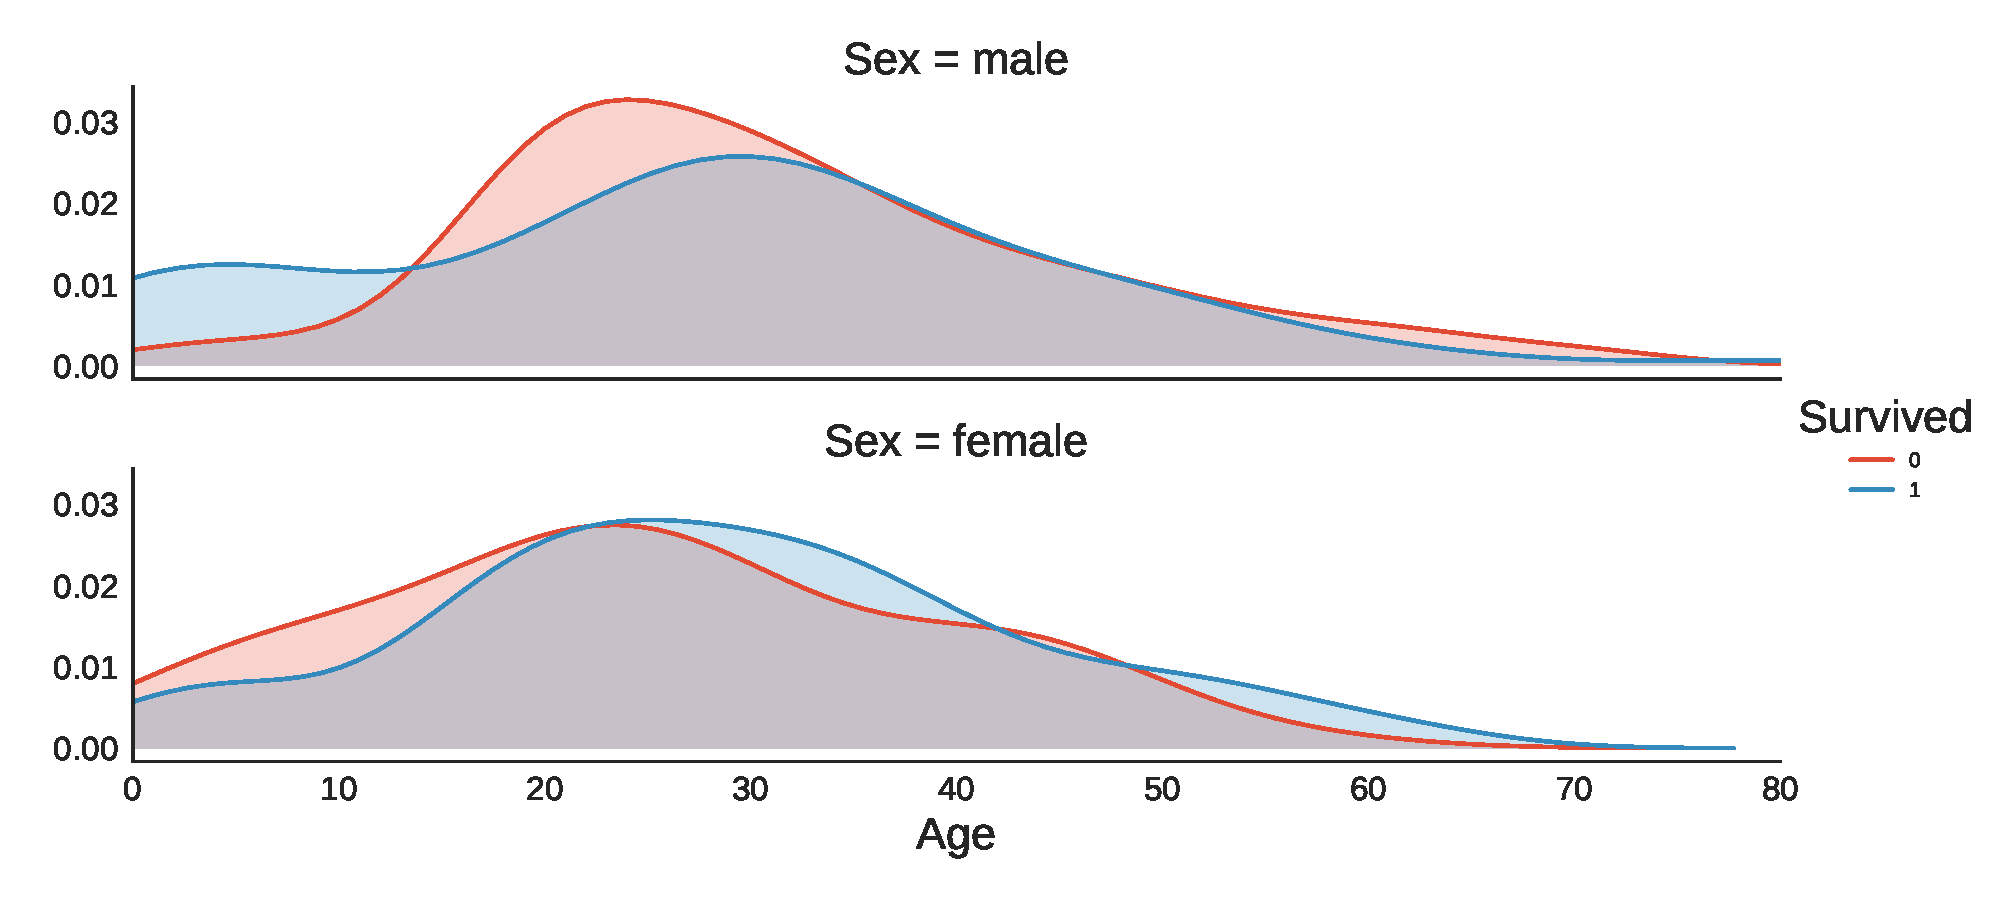
\includegraphics[width=0.7\textwidth]{media_saved/age_sex}
 \centering

     \caption{Survival probability depending on the passenger's age and sex.}
     \label{fig:ageallfeat}
 \end{figure}
 
\subsection*{Feature: Age}
\label{sec:age}
The survival distributions in function of the passengers' ages are pointed out in figure \ref{fig:agesexfeat} in the Appendix. The plot shows that children under twelve years were most likely to survive, whereas older children and young adults until about 30 years had bad chances.\\ 
If we categorize the survival distribution depending on the age additionally by the sex feature as shown in figure \ref{fig:agesexfeat}, it turns out that young male passengers were likely to survive while males between about 12 and 30 years were unlikely to survive. This effect is inverted for females. From this follows that age is a feature that can have influence on the predictions of our learning machine, especially if it is combined with the sex feature.


 
 \subsection*{Feature: Name and Title}
The given dataset also contains a list of the passenger-names that have been involved in the titanic accident. At first sight a name does not appear to be a useful feature for our survival predictions, but the name-list contains also a persons title. Figure \ref{fig:title} shows the total number of occurrences for all titles that have been found. The titles 'Mr.', 'Master', 'Mrs.' and 'Miss' are relatively common, whereas the other titles occur only infrequently. Therefore all other titles are grouped into a group named 'Res'. The figure also shows the chances of survival for people with different titles on the right-handed plot. The plot points out that a persons title has an impact on the survival odds. It is obvious that there is a correlation between the title feature and the sex and the age feature.

 \begin{figure}
 \centering
     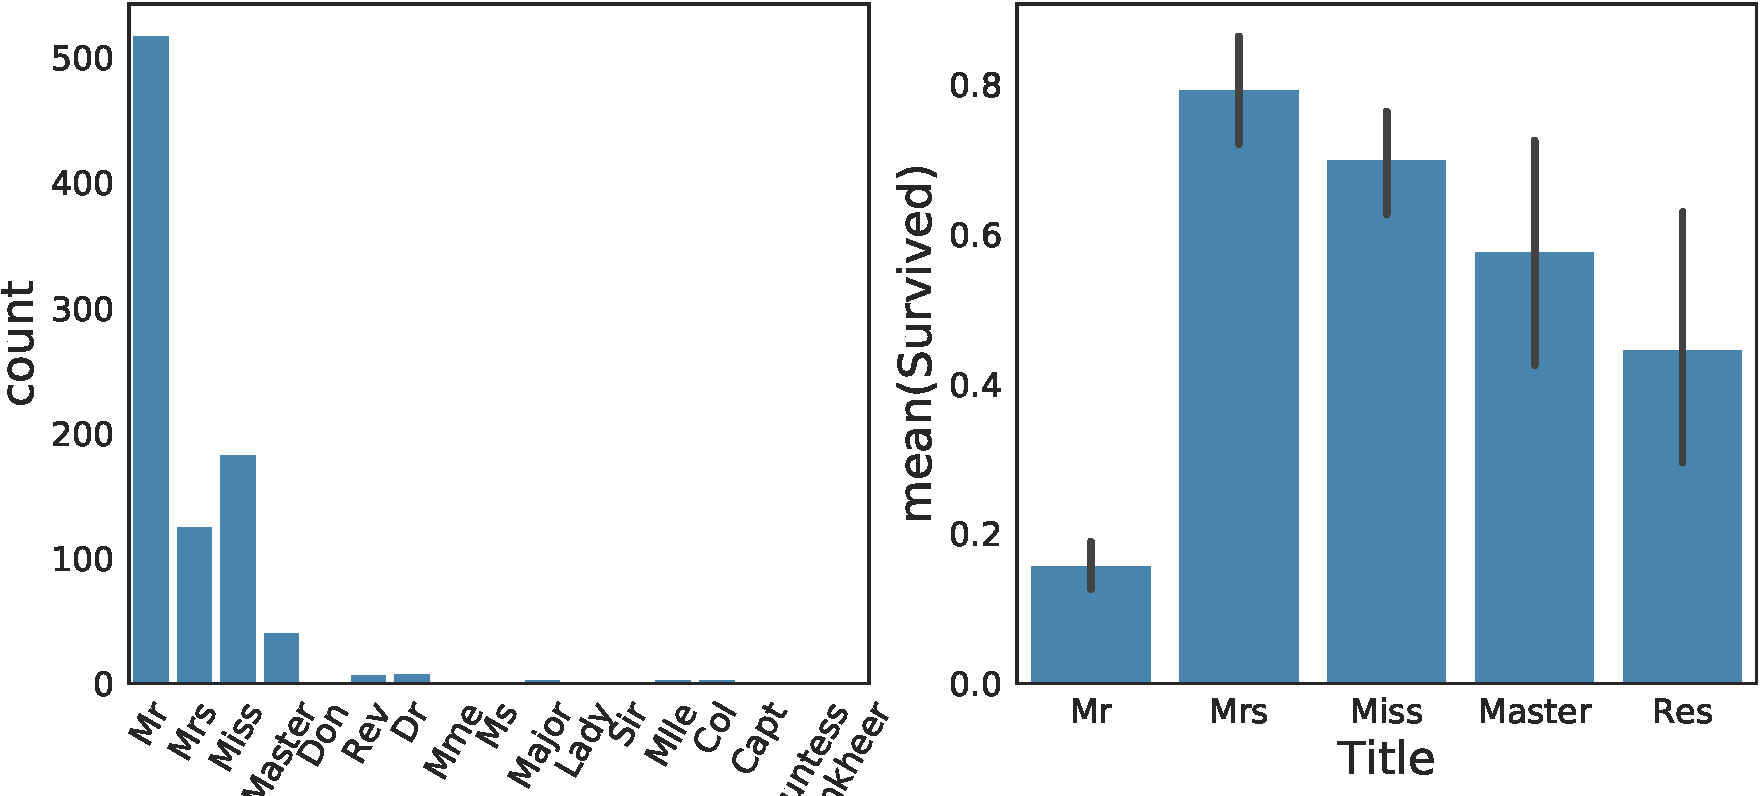
\includegraphics[width=0.5\textwidth]{media_saved/title}
     \caption{Total counts of the different titles (left) and survival probability in dependency of the title (right).}
     \label{fig:title}
 \end{figure}
 

 \subsection*{Feature: Family Constellation}
 The dataset contains two categories that handle family constellations. 'SibSp' contains the number of siblings and spouses a passenger was travelling with and 'Parch' contains the number of parents and children aboard. Figure \ref{fig:familyold} points out the influence of family constellations on the survival rate. The errorbars imply that the number of datasets with more than two siblings and spouses or more than two parents and children aboard is to sparse for reliable predictions. For this reason the two features are grouped to a new feature called 'Family' for every point in the dataset. This new feature holds the total number of a passengers relatives aboard which is grouped again into three categories containing people travelling alone, small families with one to three relatives aboard and big families with more than three relatives aboard. The classification into these groups was due to the similar survival rate of the number of relatives inside a class. The impact of the family feature is displayed in figure \ref{fig:familynew}. The the errorbars of the plot for the new feature are considerably smaller than before. In this way we can drop the 'SibSp' and the 'Parch' feature and replace it by the new family feature.
 
\begin{figure}
    \centering
    \begin{subfigure}[b]{0.48\textwidth}
     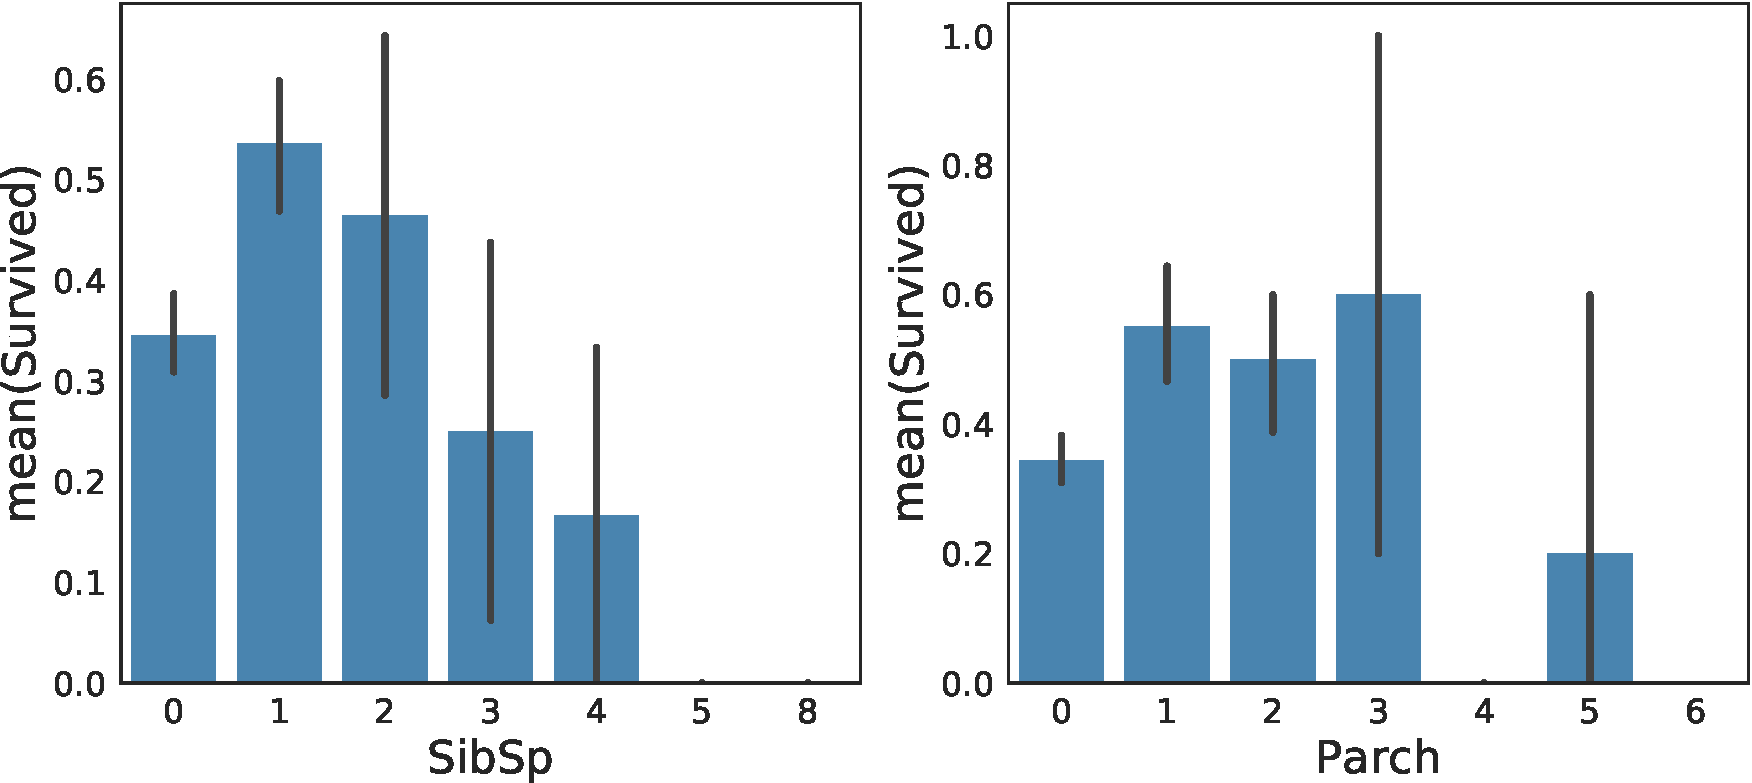
\includegraphics[width=\textwidth]{media_saved/family_size_before}
     \caption{Survival probability in dependency of the number of siblings / spouses (left) and parents / children (right) aboard.}
     \label{fig:familyold}
    \end{subfigure}
    \quad
    \begin{subfigure}[b]{0.48\textwidth}
        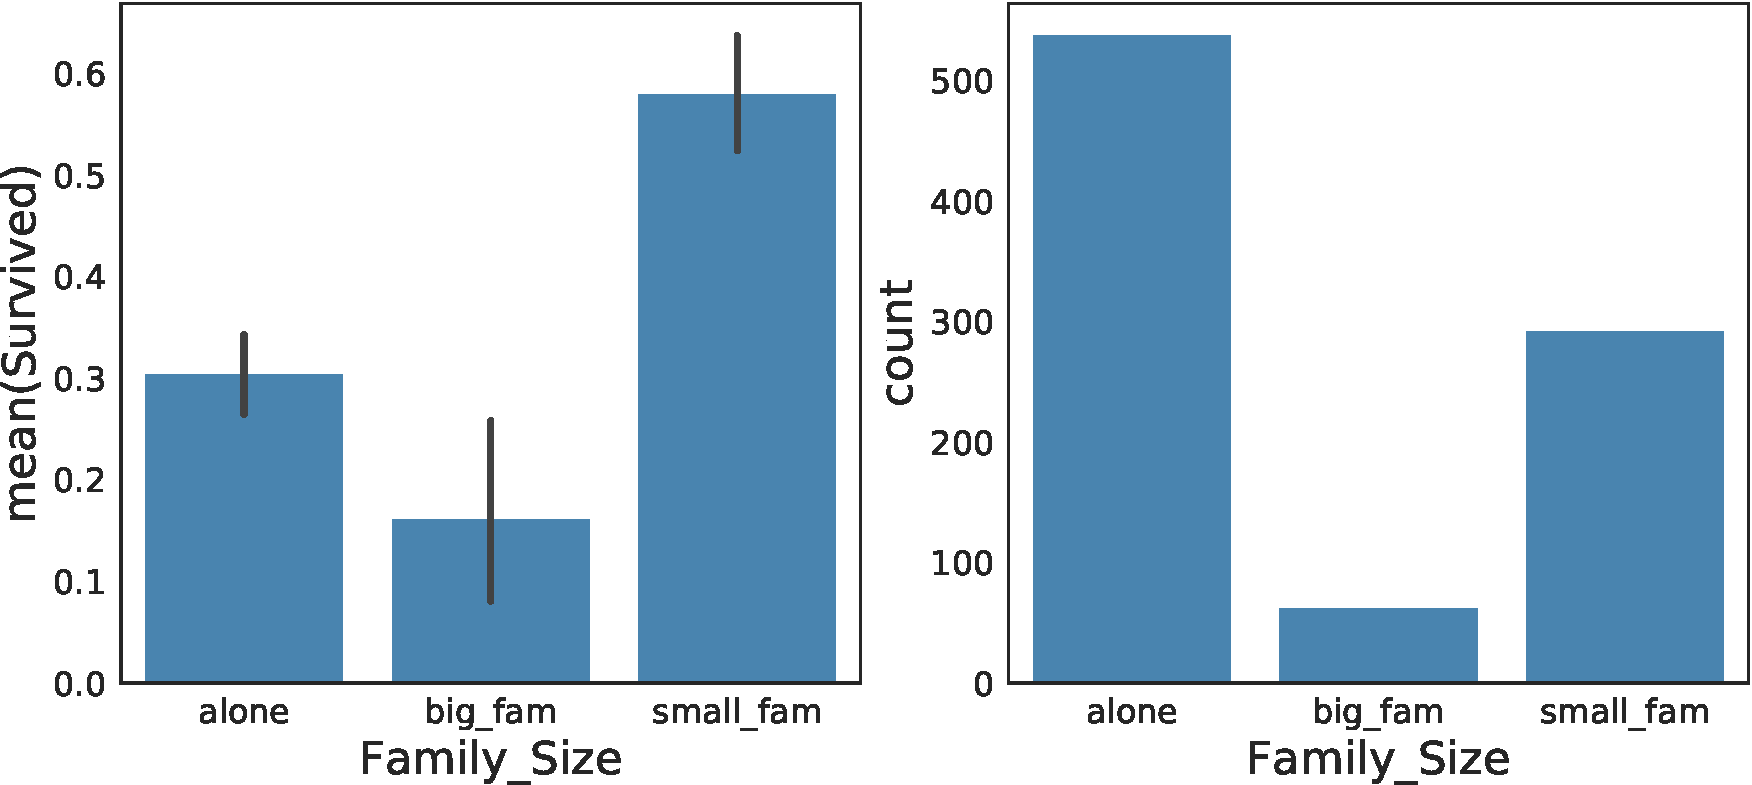
\includegraphics[width=\textwidth]{media_saved/family_size_after}
     \caption{Total number of datasets (left) survival rate (right) for the family feature.\\}
     \label{fig:familynew}
    \end{subfigure}
    \caption{Merging the SibSP and Parch feature}
\end{figure}

\begin{figure}
\centering
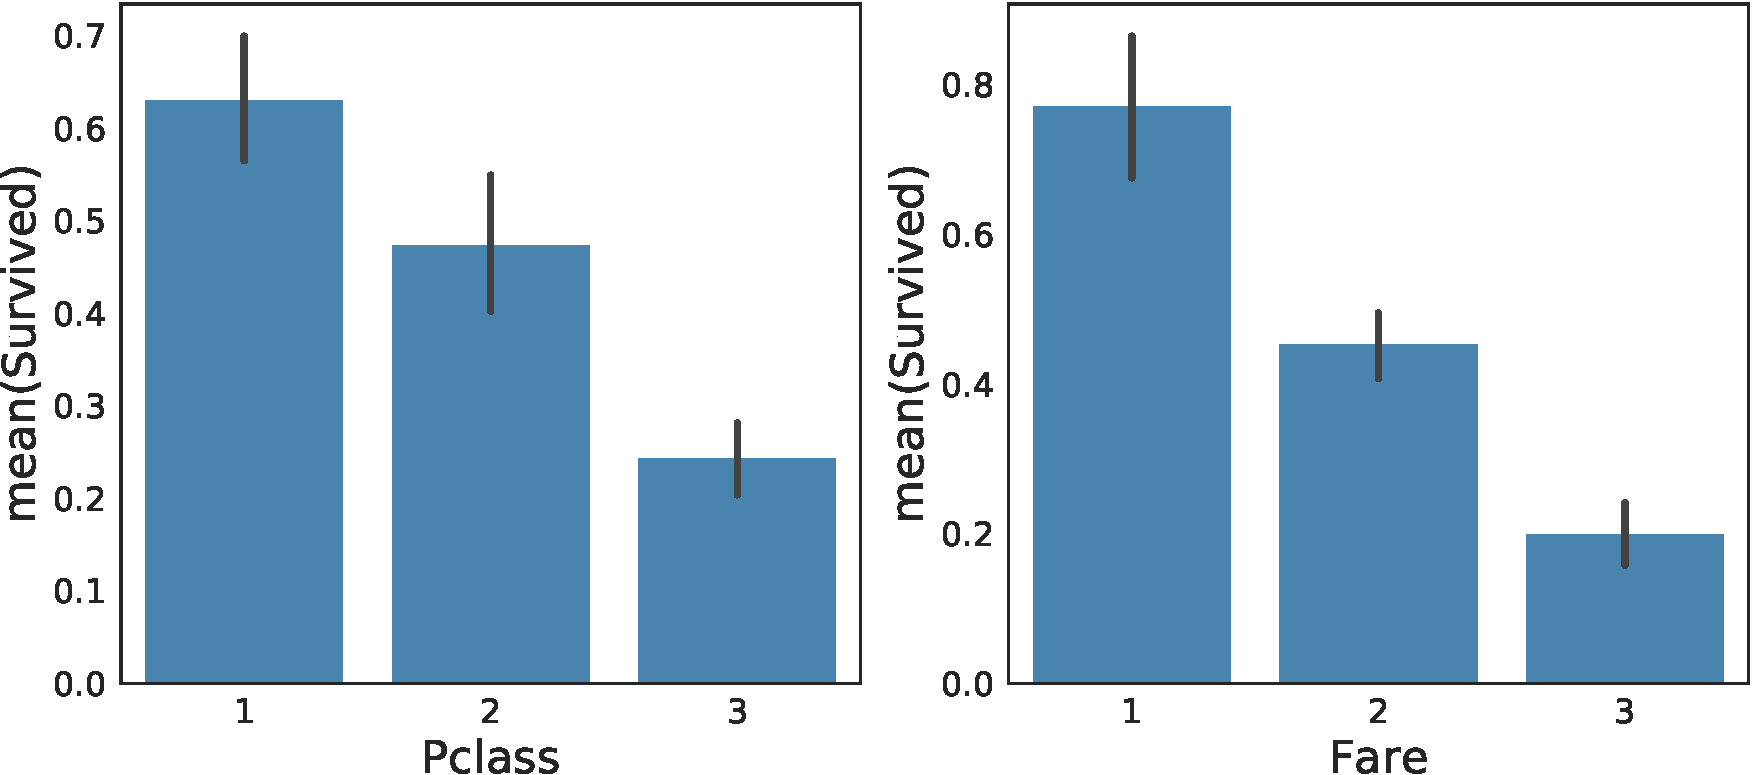
\includegraphics[width=0.5\textwidth]{media_saved/fare_survived}
     \caption{Correlation between Pclass (left), Fare (right) and survival rate.}
     \label{fig:farefeat}
\end{figure}

\subsection{Missing Data}
As already mentioned before, the dataset lacks some data for the features 'Cabin', 'Embarked' and 'Age'. In order to use these features for our learning machine it is necessary to deal with the missing data. The 'Cabin' data is mostly missing and it is not likely to find a reasonable way to estimate the data. By dividing the data into the categories 'preserved' and 'lost' as shown in figure \ref{fig:cabinfeat} it turns out that whether the data is missing or not has an effect on the survival rate. For this reason we just reclassify the feature and this already solves the missing data problem for the 'Cabin' feature. More than \mbox{99 \%} of the 'Embarked' dataset is preserved so that missing data can be discarded. Only about \mbox{80 \%} of the 'Age' data is preserved. Therefore it is worth the effort to estimate the remaining \mbox{20 \%}. As described in section \ref{sec:age} the survival rate differs for males and females in three different age categories. Additionally we can see that the age feature correlates with a passengers cabin class (see figure \ref{fig:correlationmap}) and it is obvious that a passengers title is correlated to an age. Based on this information we group all people by the titles 'Miss', 'Mrs', 'Master' and 'Mr + Res' and  furthermore by their cabin class. This leads to twelve different categories. For every category we calculate the mean age and match it to the passengers with an unknown age.\\
This way it is possible to use more than \mbox{99 \%} of our dataset without dropping a feature.

\subsection{Preparing the Dataset}
Before the dataset can be used for the training of a learning machine, all non numeric features need to be transformed into numerics. If the feature can be arranged in a meaningful order all string variables are assigned to a number. This was done for the 'Family' feature. The other features ('Sex', 'Embarked', 'Title') were transformed to a binary dataset, because they could not be arranged in a meaningful way. Afterwards the features 'SibSp', 'Parch', 'Name', 'PassengerID' and 'Ticket' were dropped, because they are not useful for our learning machine. At last we scale all features on a scale between 0 and 1, so that all features have the same influence on the predictions.

\section{Implementation of an easy SMO Algorithm}
\subsection{Brief Introduction}
To get a better understanding of what a Support Vector Machine does we decided to implement one on our own using several publications. Most of them were based on the important paper of Platt \cite{platt} where he introduced a new approach for the calculation of the Support Vectors that improves the performance a lot. This algorithm is called Sequential Minimal Optimization. Performance was not the highest priority for us but instead understandability and the costs of implementation. Therefore we implemented a less complex version of the algorithm mainly based on \cite{smo}.

As the mathematical background of the SVMs has been explained in the lecture and might be considered a standard solution for machine learning, the following introduction focuses on the main equations.

The initial problem is a linear separable dataset with the labels $y_i \in \{-1, 1\}$. The classifier that the SVM is supposed to compute will have the form

\begin{equation}
    f(x) = \langle \omega, x \rangle + b
\end{equation}

Now suppose we have a separating hyperplane and $w$ is perpendicular. The main task of the SVM is to maximise the closest perpendicular distance between the hyperplane and the two classes. This is down by the following constraints

\begin{align}
f(x) &\geq 1\ \text{for $y_i = +1$} \\
f(x) &\leq 1\ \text{for $y_i = -1$}
\end{align}

Consequently do points that lie on the hyperplane satisfy $f(x)=0$.

From these set of equations follows that the minimal distance from the hyperplane to one of the datapoints is $d=\frac{1}{|\omega|}$ which shall be maximized. Introducing an additional factor that allows but penalizes non separable noise and reformulating the problem with Lagrange multipliers (the $\alpha _i$) we get the following problem:

\begin{align}
\text{max}_\alpha& W(\alpha) = \sum_{i=1}^m \alpha _i - \frac{1}{2} \sum_{i=1}^m \sum_{j=1}^m y^{(i)} y^{(j)} \alpha _i \langle x^{(i)}, x^{(j)} \rangle \\
\text{subject to \em} & 0\leq \alpha _i \leq C, i = 1,..., m \\
& \sum_{i=1}^m \alpha _i y^{(i)} = 0 \label{eq:sumalpha}
\end{align}

For the presented problem the Kuhn Tucker conditions define the $\alpha _i$ that represent an optimal solution. The KKT conditions are

\begin{align}
\alpha _i = 0 & \implies  y^{(i)}(\langle \omega, x^{(i)}\rangle + b)  \geq 1 \\
\alpha _i = C & \implies  y^{(i)}(\langle \omega, x^{(i)} \rangle + b)  \leq 1 \\
0 \geq \alpha _i \geq C & \implies  y^{(i)}(\langle \omega, x^{(i)} \rangle + b)  = 1 \label{eq:alphabounds}
\end{align}

To deal with linearly non separable data, the scalar products can be replaced by kernel functions $kernel(x_i, x_j)$.

\subsection{Description of the Implementation}
Instead of trying to maximize the whole set of $\alpha$ the SMO algorithm exploits that the maximum will be reached when pairs $\alpha _i, \alpha _j$ fulfil the KKT conditions (while it needs to be at least a pair, since the conditions imply linearity of two $\alpha$ values). Thus the SMO algorithm selects two $\alpha$ parameters (that do not meet the KKT conditions) and optimizes them. Afterwards the threshold gets adjusted according to the new values.

A big part of the actual publication from Platt deals with the heuristic of how two choose the $\alpha _i$ and $\alpha _j$ since this is a critical factor for the pace of its convergence as the number of possible pairs in a setup with $m$ features is $m(m-1)$. Accordingly the amount of time it takes to find the \textit{critical} values is decisive for the algorithms performance.

Nevertheless, in this assignment a very simple heuristic is implemented in order to keep the code simple and understandable: the pairs are just purely randomly selected.

Fig. \ref{fig:pseudo} in the Appendix shows the pseudo code of our implementation. Basically the algorithm consists of an outer and inner loop. The inner loop iterates through the $\alpha _i$ and checks weather it violates the KKT conditions. If this is the case, randomly a second parameter $\alpha _j$ is selected and will be adjusted using that the optimal $\alpha _j$ is given by
\begin{equation}
\alpha^{'}_j = \alpha _j  - \frac{y^{(j)} (E_i - E_j)}{\eta}
\end{equation}
where $\eta$ can be interpreted as the second derivative of the generic function function $W(\alpha)$ \cite{smo}. $E_i$ is the current error on the sample $x_i$. After that the new parameter is cropped to boundaries that follow from equation \ref{eq:alphabounds} and \ref{eq:sumalpha}. Then the opposing parameter is calculated exploiting the linearity the threshold can be updated by using the classifier function $f(x)$ and either one $alpha$ that lays within $(0, C)$ or if this is true for both, their arithmetic mean.

The outer loop counts how often the inner loop fails to find a partner for optimization or the optimization yields to no significant changes (significance is defined by the user). The algorithm terminates when a certain, user defined number of passes is reached.

\subsection{Comparison with SciKit SVM}
The implementation does not make a lot use of Numpy's vectorization skills and therefore performs poor even considering that it is Python code. Still it reaches satisfying scores with the titanic train set in comparison to other SciKit algorithms as can be seen in fig. \ref{fig:comparison}.

\begin{figure}
  \centering
    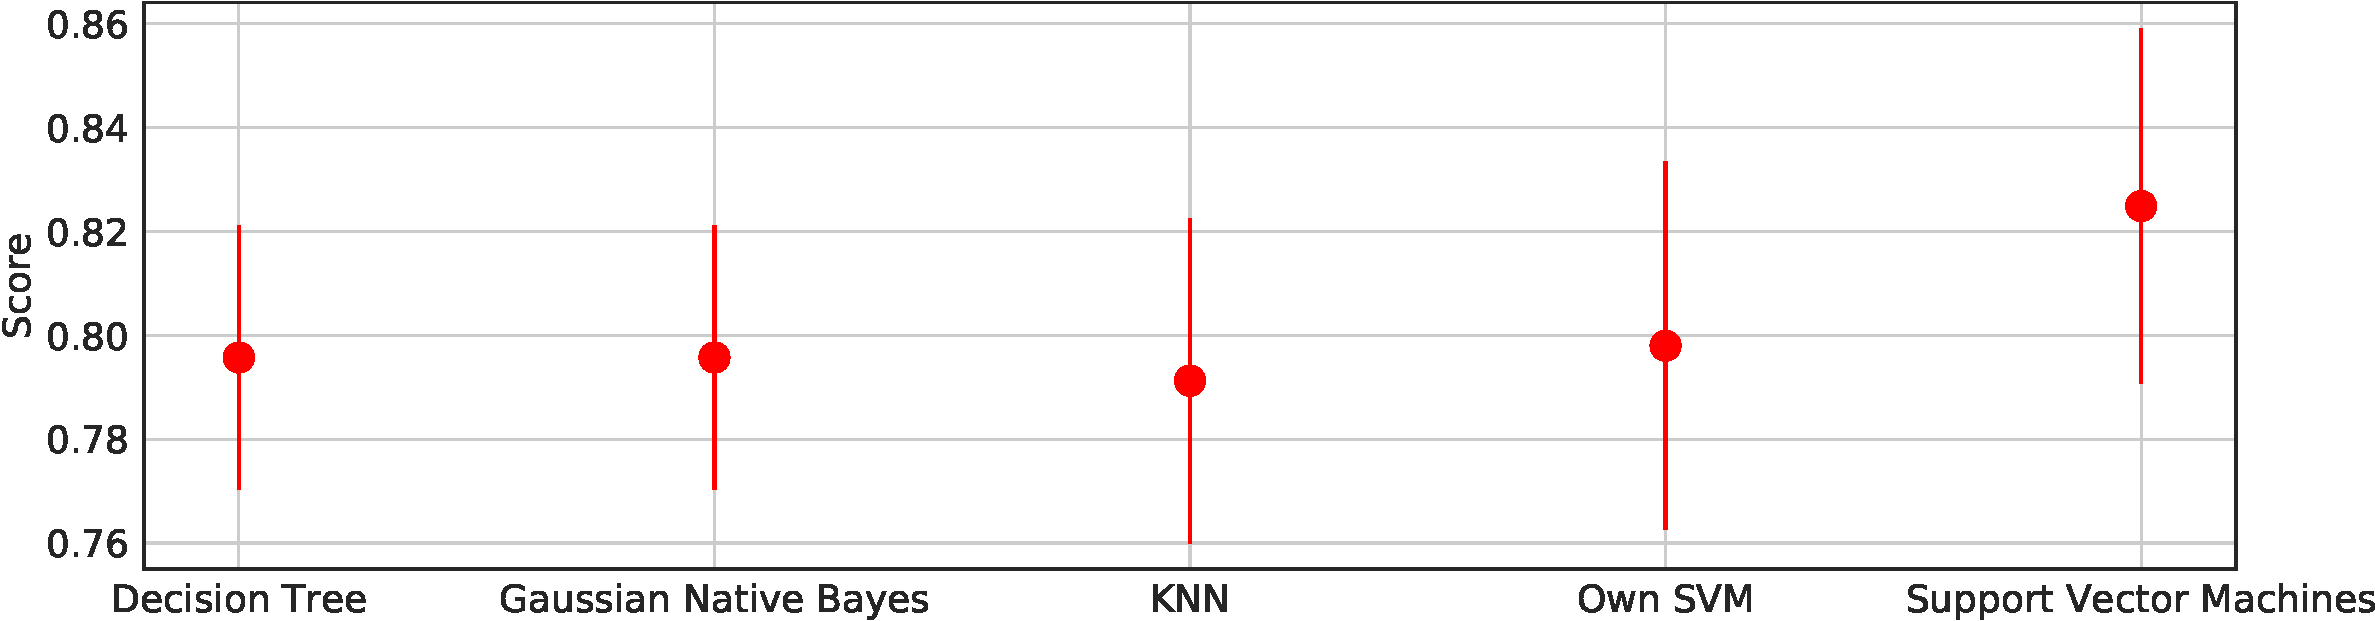
\includegraphics[width=0.8\textwidth]{media_saved/ml_comparison}
  \caption{Comparison of different ML Algorithms and their score using the Titanic training set and K-Fold validation.}  
  \label{fig:comparison}  
\end{figure}

On the other hand and less surprisingly, the performance is quite poor compared to the SVM Module from the SciKit framework\footnote{\url{http://scikit-learn.org/stable/modules/generated/sklearn.svm.SVC.html}}. One can deduce from figure \ref{fig:benchmark} that the prefactor as well as the exponential behaviour is significantly worse.

\begin{figure}
  \centering
    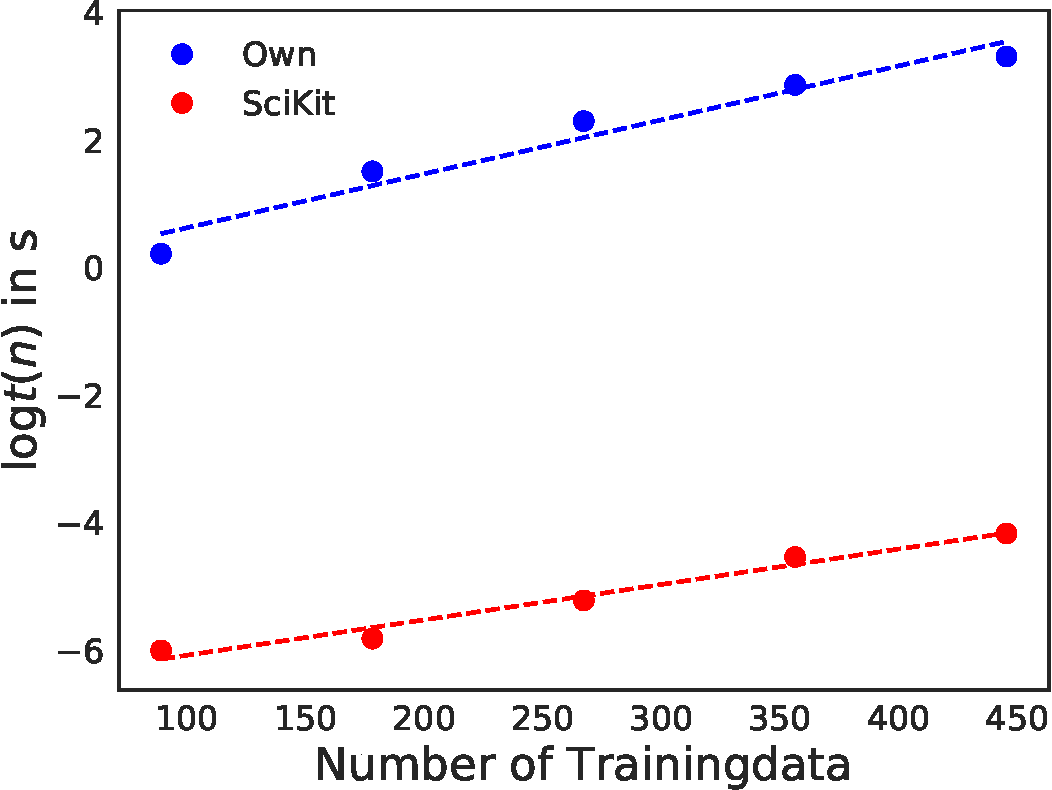
\includegraphics[width=0.4\textwidth]{media_saved/benchmark}
  \caption{Comparison the self made implementation and the optimized SciKit implementation. The different intercepts ($\Delta \approx 6$) as well as the different slopes (factor $1.6$) express the smaller prefactor and exponent of runtime of the SciKit's implementation.}  
  \label{fig:benchmark}  
\end{figure}

It turned out that the quality of the result heavily depends on the parameter that determines after how many \textit{changeless} runs it terminates. As you can see in figure \ref{fig:max_passes}, the algorithm yields a lot support vectors that do not lie within the margin when it stops after one changeless iteration. The quality of the solution increases when the number of passes is larger. The same holds for the runtime unfortunately. This behaviour results from the optimization behaviour of the SVM which is that it only optimizes data points which lay within the margin. Since this "quickly" becomes a small number of data points it is unlikely that the random selection finds a pair to optimize.

\begin{figure}
    \centering
    \begin{subfigure}[b]{0.28\textwidth}
        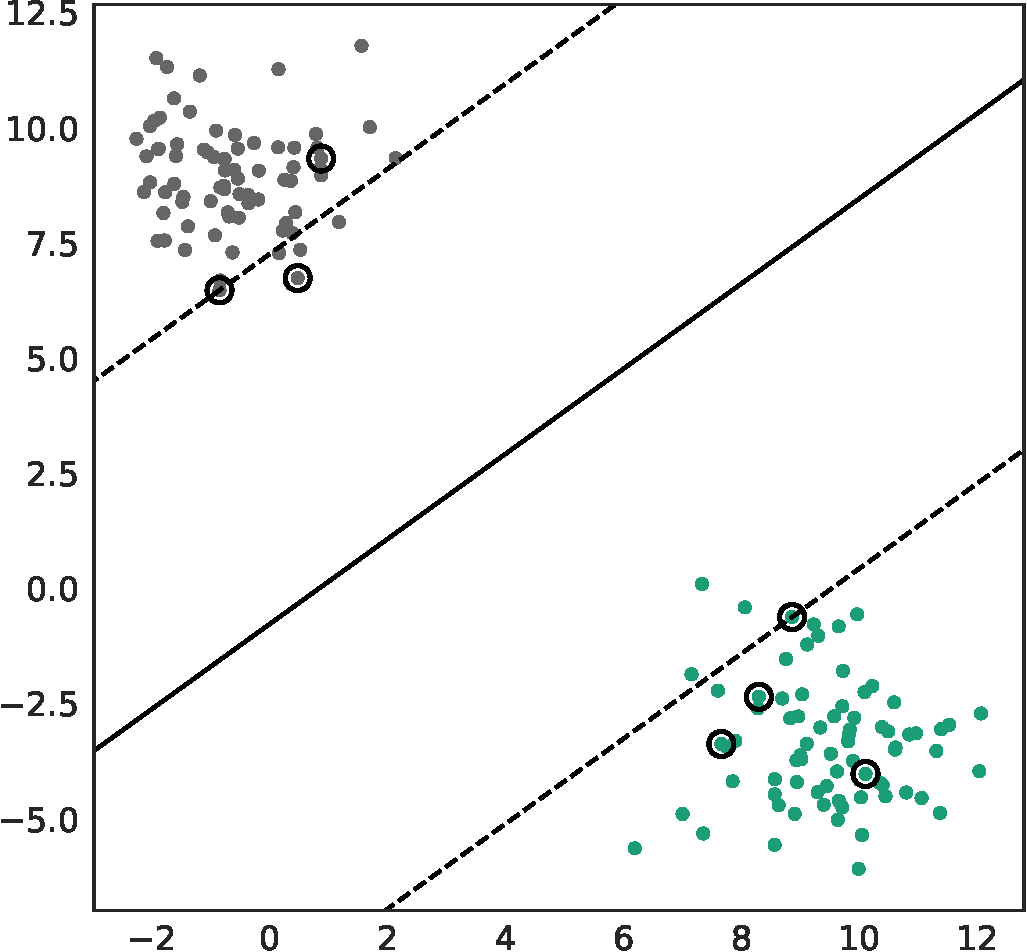
\includegraphics[width=\textwidth]{media_saved/own_test_mpasses_1.pdf}
        \caption{\texttt{max\_passes=1}}
        \label{fig:max_passs_1}
    \end{subfigure}
    \quad
    ~ %add desired spacing between images, e. g. ~, \quad, \qquad, \hfill etc. 
      %(or a blank line to force the subfigure onto a new line)
    \begin{subfigure}[b]{0.28\textwidth}
        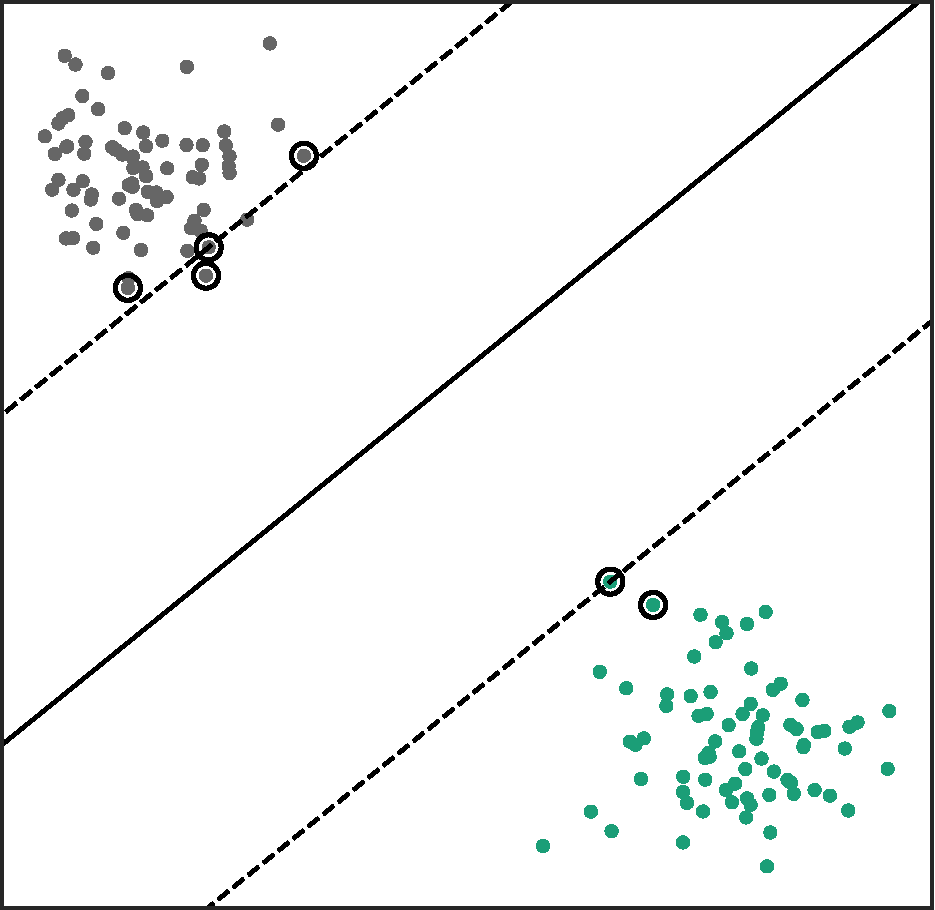
\includegraphics[width=\textwidth]{media_saved/own_test_mpasses_15.pdf}
        \caption{\texttt{max\_passes=15}}
        \label{fig:max_pass_15}
    \end{subfigure}
    \quad
    ~ %add desired spacing between images, e. g. ~, \quad, \qquad, \hfill etc. 
    %(or a blank line to force the subfigure onto a new line)
    \begin{subfigure}[b]{0.28\textwidth}
        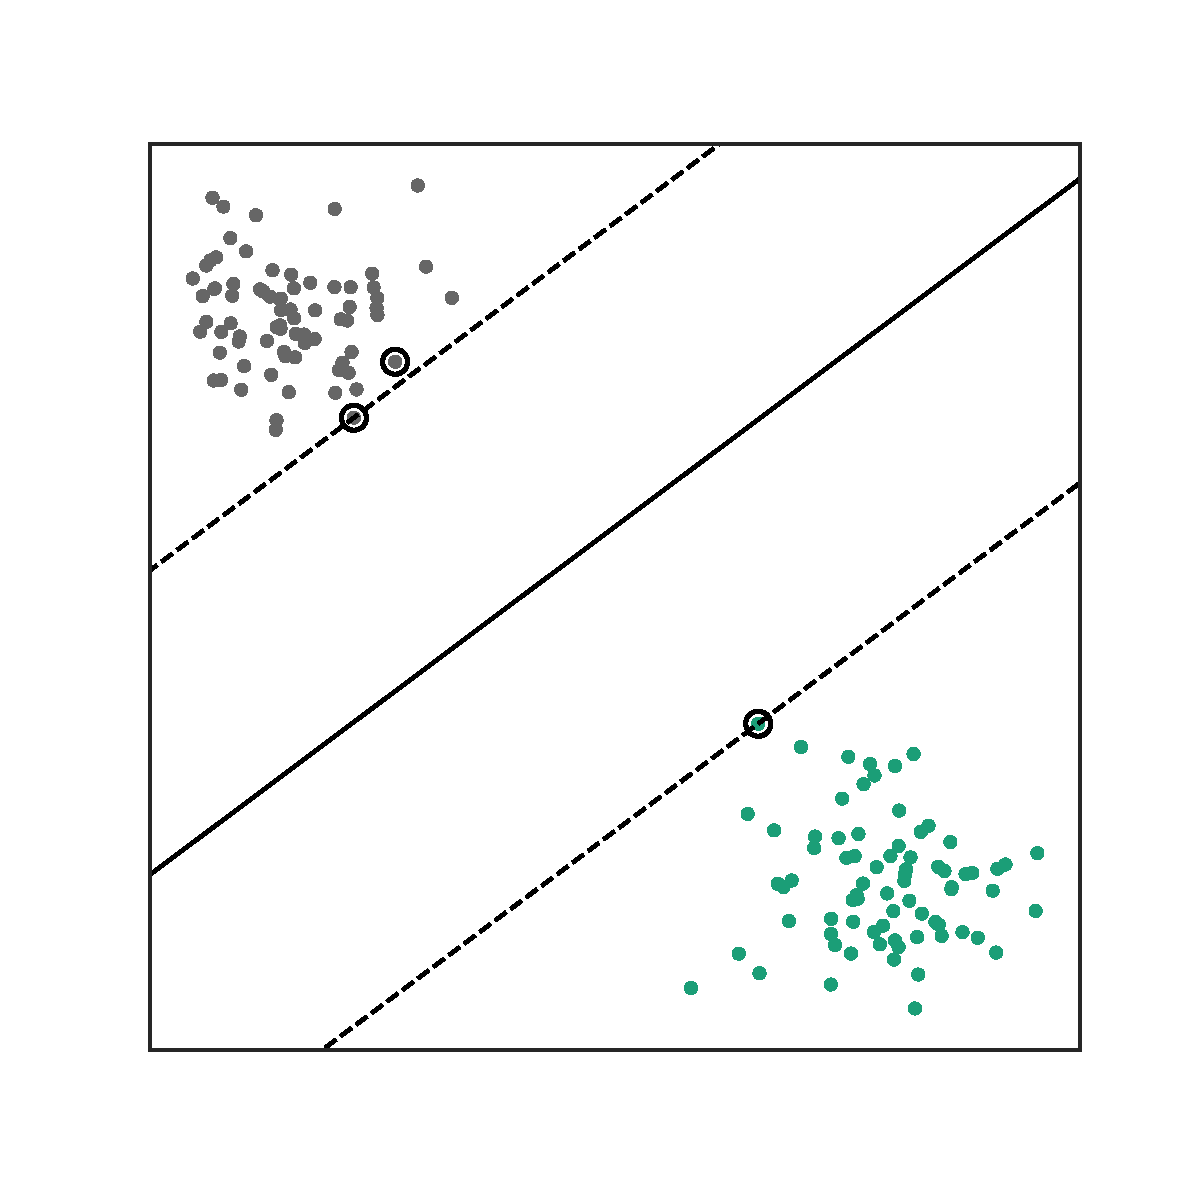
\includegraphics[width=\textwidth]{media_saved/own_test_mpasses_30.pdf}
        \caption{\texttt{max\_passes=30}}
        \label{fig:max_pass_30}
    \end{subfigure}
    \caption{Results of our SVM on a linear seperable test set depending on after how many changeless loops it terminates.}\label{fig:max_passes}
\end{figure}

\section{Summary}
We were able to apply our knowledge from class on a simple example problem and thereby extend it with practical skills such as analysing and optimizing features, using the SciKit Framework and dealing with missing data. Additionally we gained deeper insight into one Machine Learning algorithm and were able to point out one critical factor for its performance.

\clearpage
\appendix
\section*{Appendix}
\section{Figures}
 \begin{figure}[h]
 \centering
     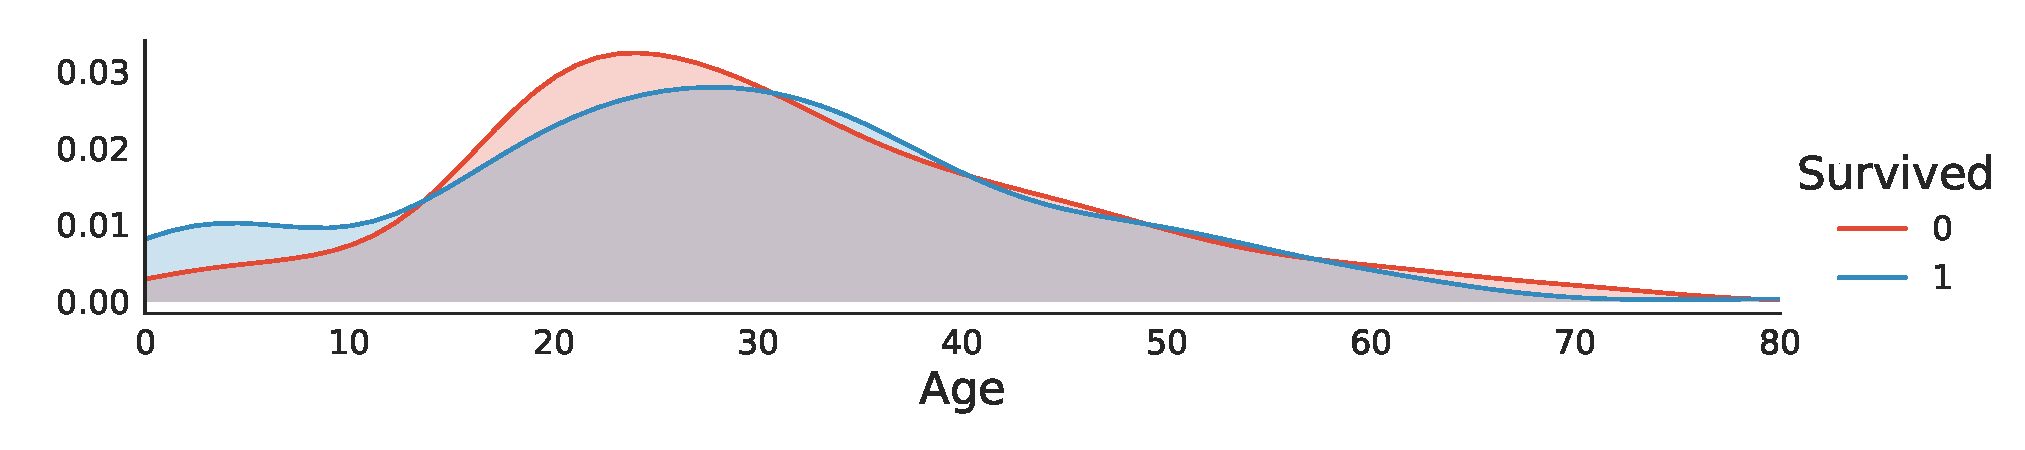
\includegraphics[width=0.8\textwidth]{media_saved/age_all}
     \caption{Survival probability depending on the passenger's age and sex.}
     \label{fig:agesexfeat}
\end{figure}
\begin{figure}[h]
\centering
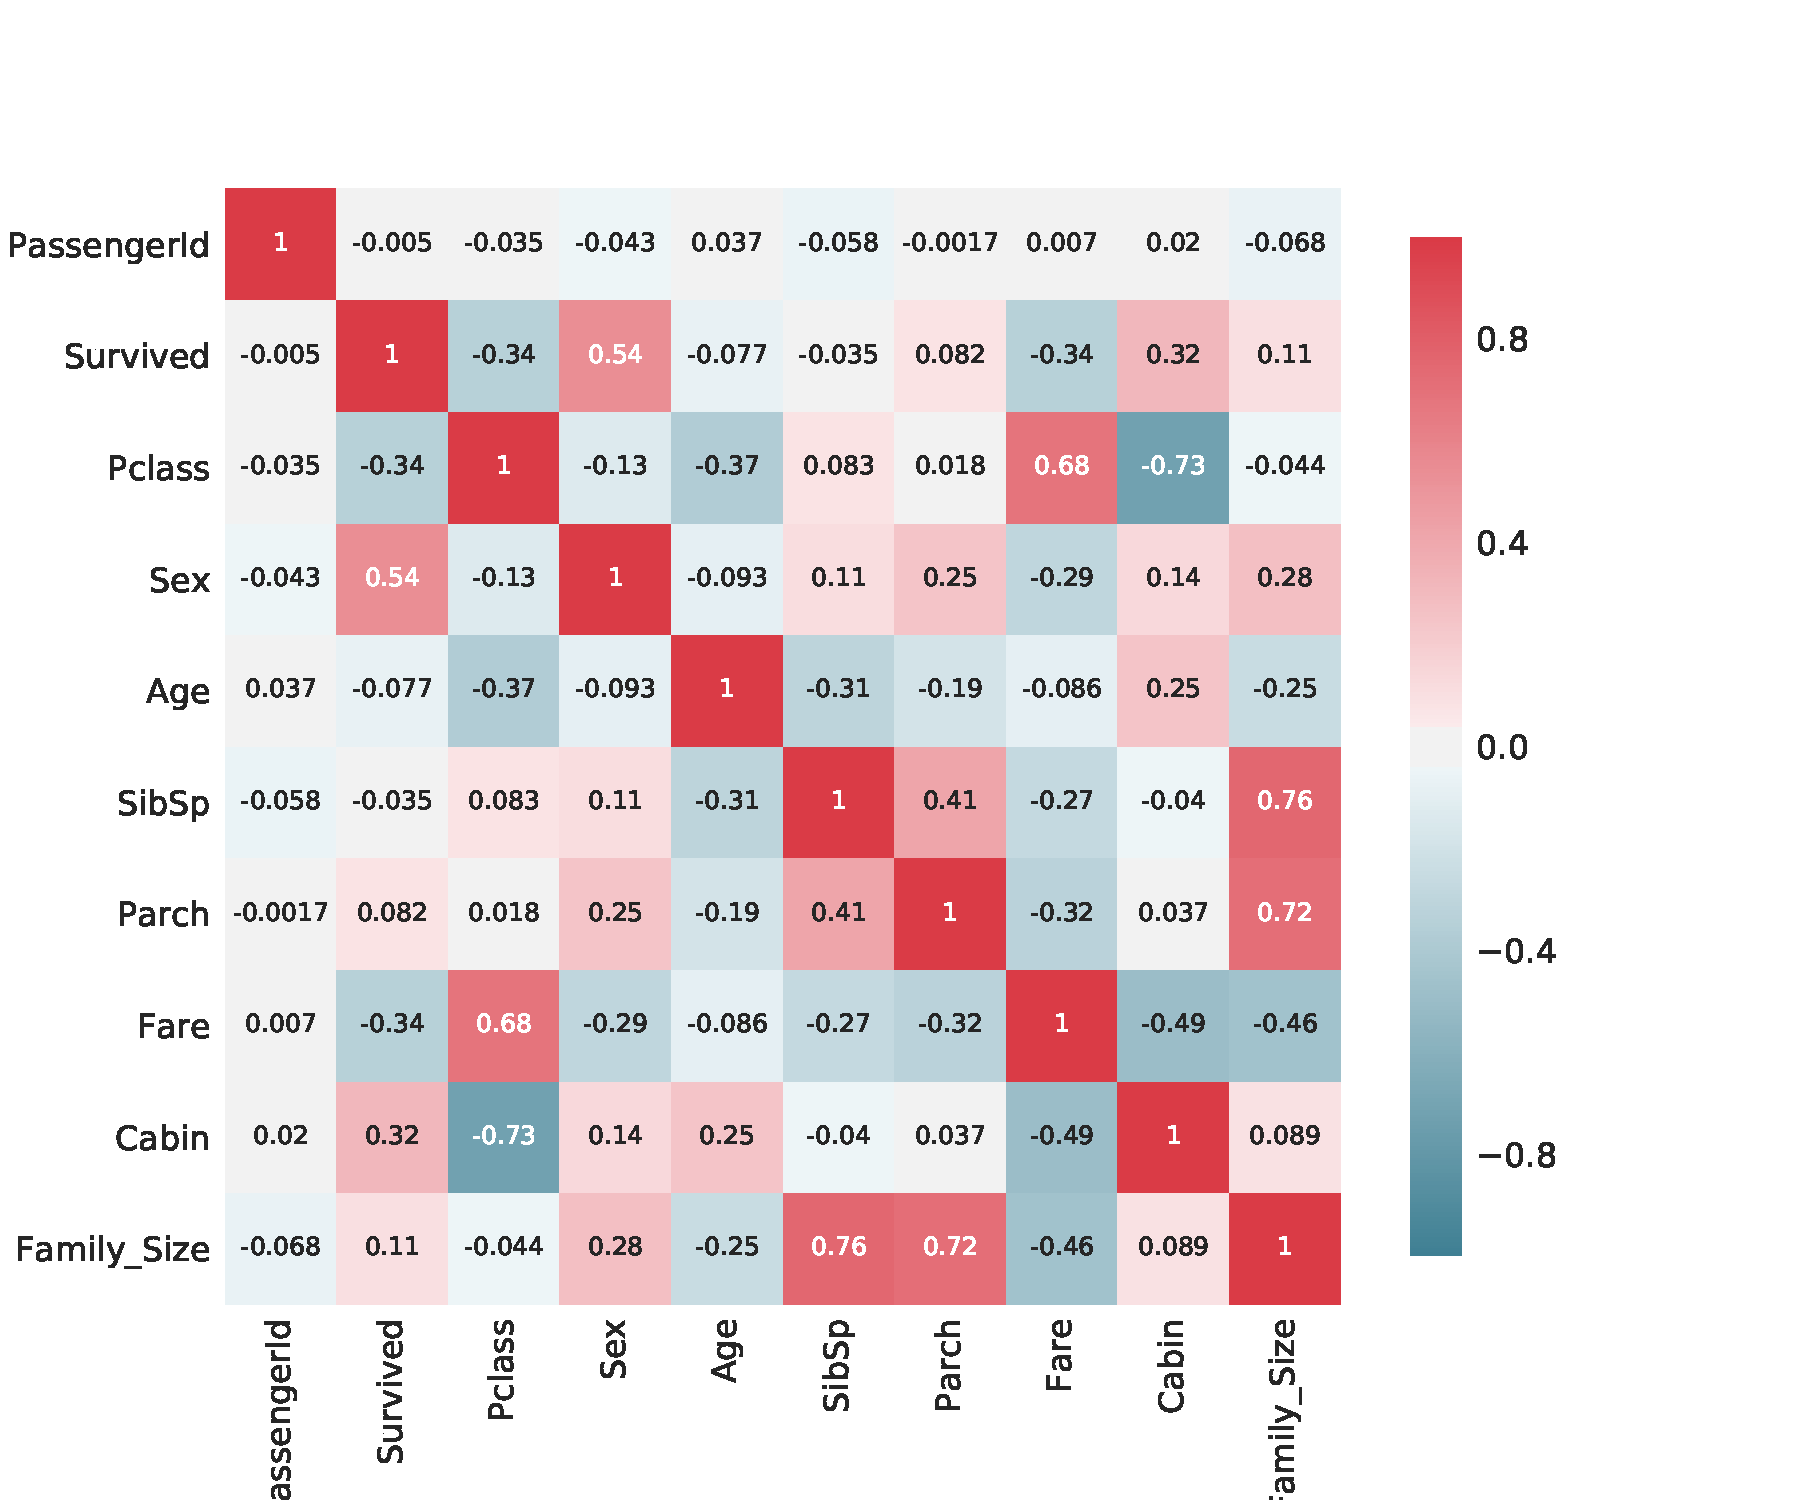
\includegraphics[width=0.9\textwidth]{media_saved/correlation_map}
     \caption{Correlation map of the dataset.}
     \label{fig:correlationmap}
\end{figure}

\newpage
\section{Pseudo Code of the SMO algorithm}
\begin{figure}[!h]
  \centering
    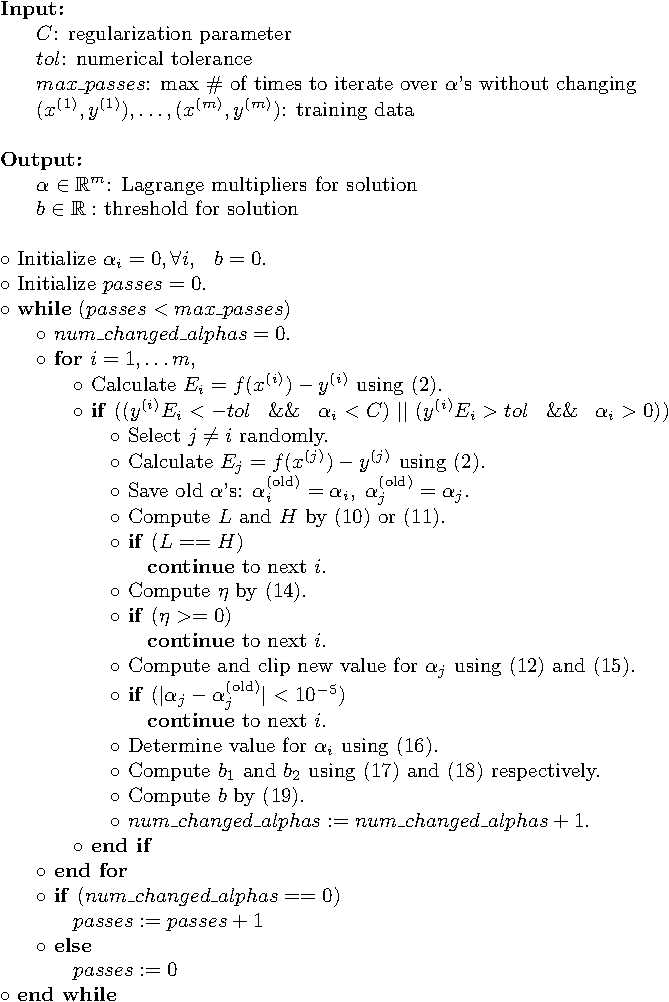
\includegraphics[width=0.8\textwidth]{media_saved/pseudo_code}
  \caption{Pseudo Code of the implemented SMO algorithm. Taken from\cite{smo}}  
  \label{fig:pseudo}  
\end{figure}

\iffalse
%%% THIS PART GETS IGNORED %%%
\section{Code}
\lstinputlisting[
	label={code},
	caption={The main procedure of the SMO algorithm},
	style=py,									% Style
	firstnumber={0},
	lastline={172},										% Start der Nummerierung
	firstline={56}											% 1. Codezeile
]											% letzte Codezeile
{./own_svm/own_svm.py}

\begin{SCfigure}
  \centering
  \includegraphics[width=0.3\textwidth]%
    {media_saved/benchmark}% picture filename
      \caption{Comparison the self made implementation and the optimized SciKit implementation. The different intercepts ($\delta ~ 6$) as well as the different slopes (factor $1.6$) express the smaller prefactor and exponent of runtime of the SciKit's implementation.}
      \label{fig:benchmark}  
\end{SCfigure}
\fi
%%% Stop ignorance %%%
\clearpage

\printbibliography %hier Bibliographie ausgeben lassen
\end{document}      